\subsection{block design}
We are interested in the simple block experiment in this research, so we are 
first to the fit block desigin to ordinary least sqaures regression in order to
define the basic relationship between neural signal and blood pressure. Here, 
we assume the error from data is followed independent and identicallynormal
distribution and constant variance.
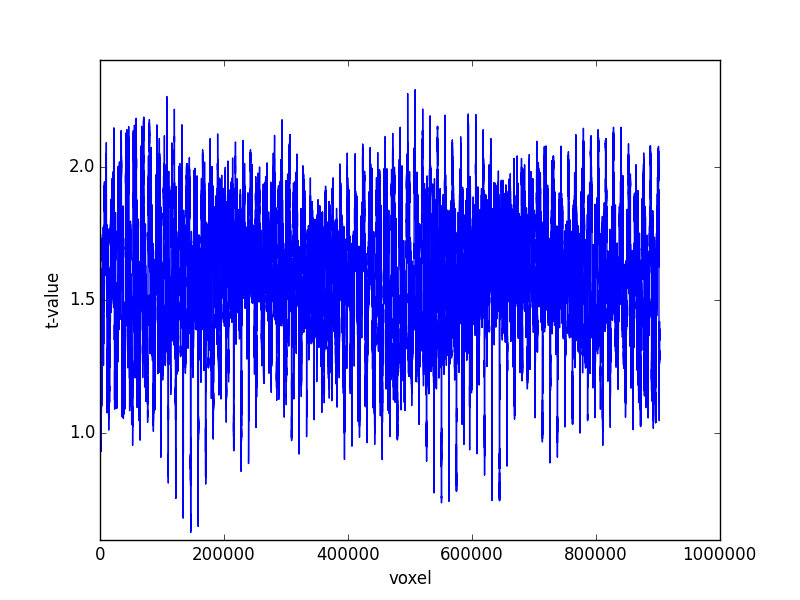
\includegraphics{task001_run001_T_value_block}
\label{T-value of $\hat{\beta_{3}}$ in block design OLS}
Since the $\hat{\beta_{3}}$ in 2 demission is not easy to recognize which voxels
are significantly active, we would like to reshape to 3 demission as the brain 
shape. Then, we plot the $\hat{\beta_{3}}$ and P-value of front, middle and 
back perspectives respectively.
\includegraphics{block_beta_front_map, block_p_front_map}
\label{Front perspective of brain in block design}
\includegraphics{block_beta_middle_map, block_p_middle_map}
\label{Middle perspective of brain in block design}





